\documentclass[11pt,a4paper]{article}
\usepackage[T1]{fontenc}\usepackage[utf8]{inputenc}\usepackage{lmodern,amsmath,amssymb,graphicx,booktabs,array,microtype,float,placeins,caption,listings,xcolor,adjustbox}
\usepackage[margin=25mm]{geometry}\usepackage[hidelinks]{hyperref}\usepackage{fancyhdr}
\pagestyle{fancy}\fancyhf{}\fancyhead[L]{Quick Return Mechanism Analysis}\fancyfoot[C]{\thepage}\setlength{\headheight}{14pt}
\setlength{\parindent}{0pt}\setlength{\parskip}{6pt}\setlength{\emergencystretch}{2em}\captionsetup{font=small,labelfont=bf}
\lstset{language=Matlab,basicstyle=\ttfamily\scriptsize,breaklines=true,columns=fullflexible,keepspaces=true,showstringspaces=false,numbers=left,numberstyle=\tiny\color{gray},frame=single,rulecolor=\color{gray!25}}
\setcounter{MaxMatrixCols}{20}\begin{document}
\begin{titlepage}\centering

\includegraphics[height=22mm]{figures/rId9.png}\hfill
\includegraphics[height=22mm]{figures/rId8.png}\par
\vspace{18mm}{\Large Machine Dynamics\par}\vspace{12mm}
{\huge\bfseries Quick Return Mechanism\par}\vspace{7mm}{\Large Kinematics Dynamics and Cam Design\par}\vspace{18mm}
{\Large Pouya Asghari\par}\vspace{10mm}Instructor: Dr. Rastgoo\par
\vfill School of Mechanical Engineering\par College of Engineering, University of Tehran\par
Second semester of academic year 1403--1404\par Submission date: 1404/03/16 (Iranian calendar)\par
\end{titlepage}
\section*{About this edition}
This is an English translation of the supplied Persian report. The analysis, reported dimensions, source equations, comparison figures, and code are retained. Mathematical notation is transcribed from the source rather than presented as independently verified equations. The student number is omitted.

The source acknowledges a discrepancy in member 5's angular velocity. The original code and native models have not been executed during translation. A separate editorial review identifies further code and reproducibility checks. Native files are preserved unchanged in the repository package; the largest MATLAB recording remains in the original archive.
\begingroup\small\setlength{\parskip}{0pt}\tableofcontents\endgroup\clearpage


\section*{Abstract}

This project focuses on the kinematic and dynamic analysis of a quick-return mechanism that converts uniform rotation into nonuniform reciprocating linear motion. A computational model is developed to determine member positions, velocities, accelerations, joint forces, and input torque. A MATLAB program simulates two motion cycles and plots angular velocities and accelerations. The dynamic analysis extends the calculation to joint forces and input torque over a nominal ten-second interval, presented as plots and a force matrix.

In the second stage, the driving crank, member 2, is replaced by a cam arrangement intended to reproduce the follower's angular displacement. A cam profile is developed and compared with the target displacement using commercial mechanism simulation. The complete mechanism is animated and modeled for comparison. The project combines analytical modeling and software simulation to investigate motion reproduction and dynamic behavior. Statements of validation in the original report refer to these software comparisons, not to physical experiments.

\textbf{Keywords:} quick-return mechanism; kinematic analysis; dynamic analysis; MATLAB; joint forces; Adams/View; cam design.

\section{Introduction}

Mechanism analysis and design are important when a machine must generate a particular motion efficiently. Quick-return mechanisms produce reciprocating motion with different forward and return speeds and are used in machine tools and mechanical transmission systems. This project examines their kinematics and dynamics and designs a cam to replace one of the original members.

The principal aim is to investigate the mechanism's motion and develop a model for predicting member velocities, accelerations, and joint forces. First, analytical kinematics are implemented in MATLAB and compared with Adams/View. Next, the dynamic analysis determines joint forces and input-crank torque. Finally, a driving member is replaced with a cam and the resulting motion is compared with the target displacement.

The report presents the analysis, design, simulation, results, and discussion step by step.

\section{Kinematic Analysis}

The link lengths and initial angles are selected to permit continuous complete motion. Angular and linear velocities and accelerations are then calculated and compared with commercial simulation.

\subsection{Initial quick-return design}

\begin{figure}[H]\centering

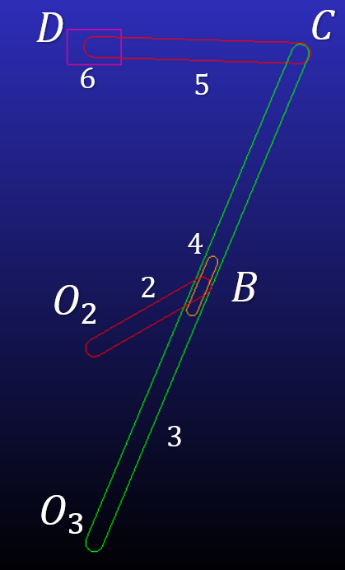
\includegraphics[width=0.85\linewidth,height=0.29\textheight,keepaspectratio]{figures/rId15.png}\par

\caption{Initial quick-return mechanism in Adams.}\end{figure}

Trial and error in Adams gives the following joint coordinates and member dimensions. Values are in meters unless otherwise indicated.

\begin{center}\begin{adjustbox}{max width=\linewidth}$\displaystyle {O}_{3}\left( 0,0\right)$\end{adjustbox}\end{center}

\begin{center}\begin{adjustbox}{max width=\linewidth}$\displaystyle {O}_{2}(0,0.11)$\end{adjustbox}\end{center}

\begin{center}\begin{adjustbox}{max width=\linewidth}$\displaystyle B\left( 0.061,0.145\right)$\end{adjustbox}\end{center}

\begin{center}\begin{adjustbox}{max width=\linewidth}$\displaystyle C\left( 0.1163,0.2765\right)$\end{adjustbox}\end{center}

\begin{center}\begin{adjustbox}{max width=\linewidth}$\displaystyle D(0,0.28)$\end{adjustbox}\end{center}

\begin{center}\begin{adjustbox}{max width=\linewidth}$\displaystyle \bar{C{O}_{3}}=0.3 \angle 67.184^\circ $\end{adjustbox}\end{center}

\begin{center}\begin{adjustbox}{max width=\linewidth}$\displaystyle \bar{B{O}_{2}}=0.07 \angle 30^\circ $\end{adjustbox}\end{center}

\begin{center}\begin{adjustbox}{max width=\linewidth}$\displaystyle \bar{DC}=0.1164$\end{adjustbox}\end{center}

All regular links have a width of 0.01 m and depth of 0.008 m. Gravity is enabled in the simulation because it is also included in the analytical calculations.

\begin{figure}[H]\centering

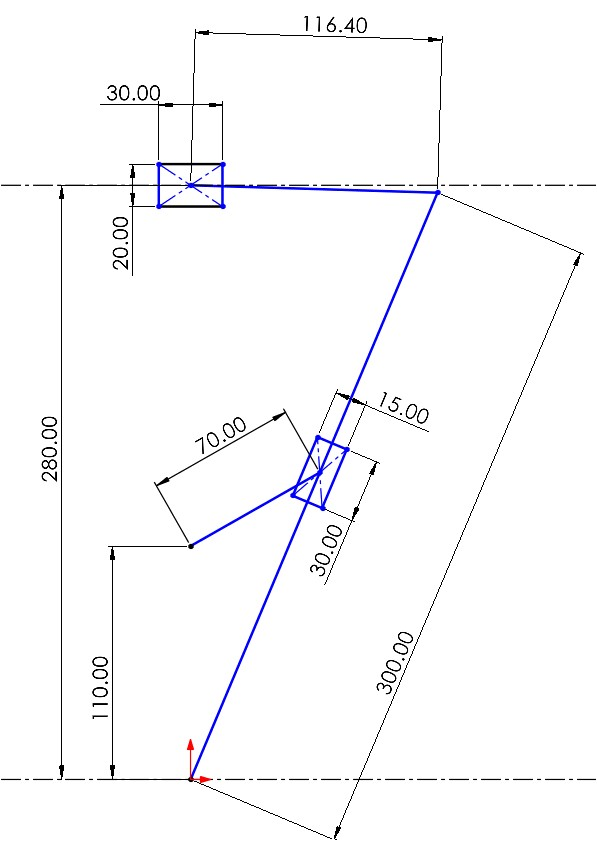
\includegraphics[width=0.85\linewidth,height=0.29\textheight,keepaspectratio]{figures/rId16.png}\par

\caption{Member dimensions; drawing dimensions are in millimeters.}\end{figure}

Member 2 is pinned to slider 4, which slides along member 3. Slider 4 must be wider than member 3; its external width is chosen as 15 mm and depth as 12 mm.

\subsection{Vector loop technique}

Two vector loops are defined for position, velocity, and acceleration analysis. The lower loop contains the fixed ground vector, the input crank vector, and the variable vector along the slotted member. The ground vector is known, and the crank length and input angle are prescribed, allowing the remaining vector length and angle to be found. Differentiating once and twice gives angular velocity, slider velocity, angular acceleration, and slider acceleration; the crank angular acceleration is zero. The upper loop includes the crank, the remaining portion of member 3, connecting member 5, a fixed vertical ground segment, and a variable horizontal displacement. The complementary member-3 segment is related to the lower-loop vector by reversing direction and subtracting its length from the total member length. The unknowns are member 5's angle and the output displacement. They are solved in the same manner. The source reuses several ground-vector symbols; the diagram and supplied code clarify their roles.

\begin{figure}[H]\centering

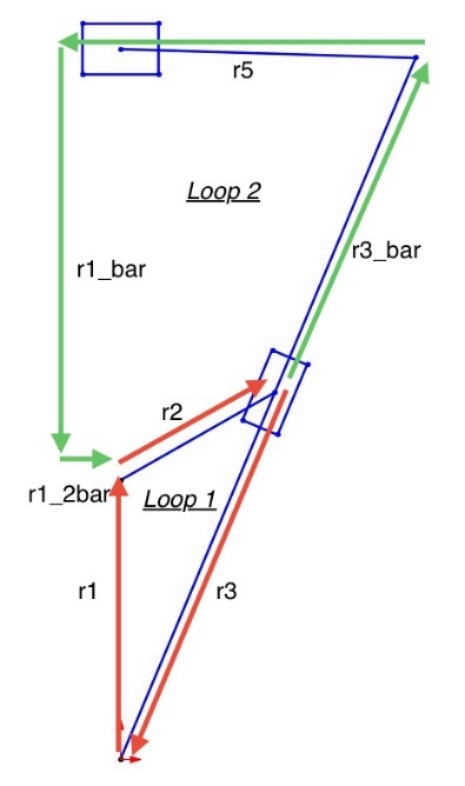
\includegraphics[width=0.85\linewidth,height=0.29\textheight,keepaspectratio]{figures/rId17.png}\par

\caption{Vector loops used in the analytical model.}\end{figure}

\subsection{Vector equations}

The general approach is implemented using the following complex-vector loop equations. Original mathematical notation is retained; ambiguities and potential errors require checking against the code.

\textbf{Loop I}

\begin{center}\begin{adjustbox}{max width=\linewidth}$\displaystyle {r}_{1}+{r}_{2}+{r}_{3}=0\rightarrow {r}_{1}{e}^{i{\theta }_{1}}+{r}_{2}{e}^{i{\theta }_{2}}+{r}_{3}{e}^{i{\theta }_{3}}=0\rightarrow {r}_{3},{\theta }_{3}=determined$\end{adjustbox}\end{center}

\begin{center}\begin{adjustbox}{max width=\linewidth}$\displaystyle \frac{d}{dt}\rightarrow i{r}_{1}{\dot{\theta }}_{1}{e}^{i{\theta }_{1}}+i{r}_{2}{\dot{\theta }}_{2}{e}^{i{\theta }_{2}}+i{r}_{3}{\dot{\theta }}_{3}{e}^{i{\theta }_{3}}+{\dot{r}}_{3}{e}^{i{\theta }_{3}}=0\rightarrow {\dot{\theta }}_{3},{\dot{r}}_{3}=determined$\end{adjustbox}\end{center}

\begin{center}\begin{adjustbox}{max width=\linewidth}$\displaystyle \frac{d}{dt}\rightarrow i{\dot{r}}_{2}{\dot{\theta }}_{2}{e}^{i{\theta }_{2}}+i{r}_{2}\left( {\ddot{\theta }}_{2}+{\dot{\theta }}_{2}^{2}\right){e}^{i{\theta }_{2}}+2i{\dot{r}}_{3}{\dot{\theta }}_{3}{e}^{i{\theta }_{3}}+i{r}_{3}\left( {\ddot{\theta }}_{3}+{\dot{\theta }}_{3}^{2}\right){e}^{i{\theta }_{3}}+{\ddot{r}}_{3}{e}^{i{\theta }_{3}}=0$\end{adjustbox}\end{center}

\begin{center}\begin{adjustbox}{max width=\linewidth}$\displaystyle \rightarrow {\ddot{\theta }}_{3},{\ddot{r}}_{3}=determined$\end{adjustbox}\end{center}

\textbf{Loop II}

\begin{center}\begin{adjustbox}{max width=\linewidth}$\displaystyle {\bar{r}}_{1}+{\bar{r}}_{1}+{r}_{2}+{\bar{r}}_{3}+{r}_{5}=0\rightarrow {\bar{r}}_{1}{e}^{i{\bar{\theta }}_{1}}+{\bar{r}}_{1}{e}^{i{\bar{\theta }}_{1}}+{r}_{2}{e}^{i{\theta }_{2}}+{\bar{r}}_{3}{e}^{i{\bar{\theta }}_{3}}+{r}_{5}{e}^{i{\theta }_{5}}=0$\end{adjustbox}\end{center}

\begin{center}\begin{adjustbox}{max width=\linewidth}$\displaystyle \rightarrow {\bar{r}}_{1},{\theta }_{5}=determined$\end{adjustbox}\end{center}

\begin{center}\begin{adjustbox}{max width=\linewidth}$\displaystyle \frac{d}{dt}\rightarrow i{\bar{r}}_{1}{\dot{\bar{\theta }}}_{1}{e}^{i{\bar{\theta }}_{1}}+{\dot{\bar{r}}}_{1}+i{r}_{2}{\dot{\theta }}_{2}{e}^{i{\theta }_{2}}+\dot{{\bar{r}}_{3}}{e}^{i{\bar{\theta }}_{3}}+{i\bar{r}}_{3}{\dot{\theta }}_{3}{e}^{i{\bar{\theta }}_{3}}+i{r}_{5}{\dot{\theta }}_{5}{e}^{i{\theta }_{5}}=0$\end{adjustbox}\end{center}

\begin{center}\begin{adjustbox}{max width=\linewidth}$\displaystyle \rightarrow \dot{{\bar{r}}_{1}},\dot{{\theta }_{5}}=determined$\end{adjustbox}\end{center}

\begin{center}\begin{adjustbox}{max width=\linewidth}$\displaystyle \frac{d}{dt}\rightarrow {\ddot{\bar{r}}}_{1}+i{r}_{2}\left( i{\dot{\theta }}_{2}^{2}{e}^{i{\theta }_{2}}\right)+{\ddot{\bar{r}}}_{3}{e}^{i{\bar{\theta }}_{3}}+{2i\dot{\bar{r}}}_{3}{\dot{\theta }}_{3}{e}^{i{\bar{\theta }}_{3}}+i{\bar{r}}_{3}({\ddot{\theta }}_{3}+{\dot{\theta }}_{3}^{2}){e}^{i{\bar{\theta }}_{3}}+i{r}_{5}({\ddot{\theta }}_{5}+{\dot{\theta }}_{5}^{2}){e}^{i{\theta }_{5}}=0\rightarrow {\ddot{\bar{r}}}_{1},\ddot{{\theta }_{5}}=determined$\end{adjustbox}\end{center}

Each complex equation can be separated into real and imaginary equations and solved. This determines the mechanism's kinematic quantities.

The equations are solved in MATLAB. The source reports that vpasolve requires approximately 5--10 minutes, whereas a Newton--Raphson implementation using a Jacobian reduces the runtime to below ten seconds. These are reported timings, not independently repeated benchmarks. Newton--Raphson requires initial conditions. The MATLAB input angle begins at zero and spans two revolutions, whereas the previously illustrated geometry begins at 30 degrees. SolidWorks is therefore used to determine the dimensions and angles for a zero-degree initial crank position.

\begin{figure}[H]\centering

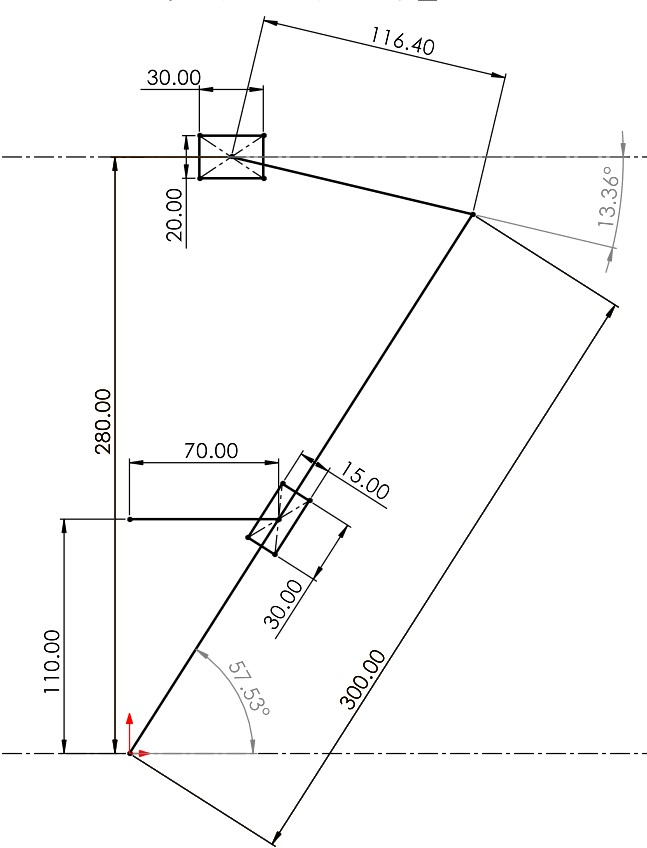
\includegraphics[width=0.85\linewidth,height=0.29\textheight,keepaspectratio]{figures/rId18.png}\par

\caption{Geometry for the zero-degree initial crank angle.}\end{figure}

The initial conditions are introduced into the solution procedure. The known and unknown quantities are arranged as follows.

\textbf{Loop I}

\begin{center}\begin{adjustbox}{max width=\linewidth}$\displaystyle \left\{ \begin{gathered}{r}_{1}cos{\theta }_{1}+{r}_{2}cos{\theta }_{2}+{r}_{3}cos{\theta }_{3}=0\\{r}_{1}sin{\theta }_{1}+{r}_{2}sin{\theta }_{2}+{r}_{3}sin{\theta }_{3}=0\end{gathered}\right.$\end{adjustbox}\end{center}

\begin{center}\begin{adjustbox}{max width=\linewidth}$\displaystyle \frac{d}{dt}\rightarrow \left\{ \begin{gathered}-{r}_{2}{\dot{\theta }}_{2}sin{\theta }_{2}+{\dot{r}}_{3}cos{\theta }_{3}-{r}_{3}{\dot{\theta }}_{3}sin{\theta }_{3}=0\\{r}_{2}{\dot{\theta }}_{2}cos{\theta }_{2}+{\dot{r}}_{3}sin{\theta }_{3}+{r}_{3}{\dot{\theta }}_{3}cos{\theta }_{3}=0\end{gathered}\right.$\end{adjustbox}\end{center}

\begin{center}\begin{adjustbox}{max width=\linewidth}$\displaystyle \rightarrow \left\{ \begin{gathered}-{r}_{2}sin{\theta }_{2}+{\dot{r}}_{3}'cos{\theta }_{3}-{r}_{3}{\dot{\theta }}_{3}'sin{\theta }_{3}=0\\{r}_{2}cos{\theta }_{2}+{\dot{r}}_{3}'sin{\theta }_{3}+{r}_{3}{\dot{\theta }}_{3}'cos{\theta }_{3}=0\end{gathered}\right.$\end{adjustbox}\end{center}

\begin{center}\begin{adjustbox}{max width=\linewidth}$\displaystyle \rightarrow \left[ \begin{matrix}cos{\theta }_{3} & -{r}_{3}sin{\theta }_{3}\\sin{\theta }_{3} & {r}_{3}cos{\theta }_{3}\end{matrix}\right]\left[ \begin{gathered}{\dot{r}}_{3}'\\{\dot{\theta }}_{3}'\end{gathered}\right]=\left[ \begin{gathered}{r}_{2}sin{\theta }_{2}\\-{r}_{2}cos{\theta }_{2}\end{gathered}\right]$\end{adjustbox}\end{center}

\begin{center}\begin{adjustbox}{max width=\linewidth}$\displaystyle \frac{d}{dt}\rightarrow \left\{ \begin{gathered}-{r}_{2}{\dot{\theta }}_{2}^{2}cos{\theta }_{2}+{\ddot{r}}_{3}cos{\theta }_{3}-2{\dot{r}}_{3}{\dot{\theta }}_{3}sin{\theta }_{3}-{r}_{3}\left( {\ddot{\theta }}_{3}sin{\theta }_{3}+{\dot{\theta }}_{3}^{2}cos{\theta }_{3}\right)=0\\-{r}_{2}{\dot{\theta }}_{2}^{2}sin{\theta }_{2}+{\ddot{r}}_{3}sin{\theta }_{3}+2{\dot{r}}_{3}{\dot{\theta }}_{3}cos{\theta }_{3}+{r}_{3}\left( {\ddot{\theta }}_{3}cos{\theta }_{3}-{\dot{\theta }}_{3}^{2}sin{\theta }_{3}\right)=0\end{gathered}\right.$\end{adjustbox}\end{center}

\begin{center}\begin{adjustbox}{max width=\linewidth}$\displaystyle \rightarrow \left\{ \begin{gathered}-{r}_{2}cos{\theta }_{2}+{\ddot{r}}_{3}'cos{\theta }_{3}-2{\dot{r}}_{3}{\dot{\theta }}_{3}sin{\theta }_{3}-{r}_{3}\left( {\ddot{\theta }}_{3}'sin{\theta }_{3}+{\dot{\theta }}_{3}^{2}cos{\theta }_{3}\right)=0\\-{r}_{2}sin{\theta }_{2}+{\ddot{r}}_{3}'sin{\theta }_{3}+2{\dot{r}}_{3}{\dot{\theta }}_{3}cos{\theta }_{3}+{r}_{3}\left( {\ddot{\theta }}_{3}'cos{\theta }_{3}-{\dot{\theta }}_{3}^{2}sin{\theta }_{3}\right)=0\end{gathered}\right.$\end{adjustbox}\end{center}

\begin{center}\begin{adjustbox}{max width=\linewidth}$\displaystyle \rightarrow \left[ \begin{matrix}cos{\theta }_{3} & -{r}_{3}sin{\theta }_{3}\\sin{\theta }_{3} & {r}_{3}cos{\theta }_{3}\end{matrix}\right]\left[ \begin{gathered}{\ddot{r}}_{3}'\\{\ddot{\theta }}_{3}'\end{gathered}\right]=\left[ \begin{gathered}{r}_{2}cos{\theta }_{2}+2{\dot{r}}_{3}{\dot{\theta }}_{3}sin{\theta }_{3}+{r}_{3}{\dot{\theta }}_{3}^{2}cos{\theta }_{3}\\{r}_{2}sin{\theta }_{2}-2{\dot{r}}_{3}{\dot{\theta }}_{3}cos{\theta }_{3}+{r}_{3}{\dot{\theta }}_{3}^{2}sin{\theta }_{3}\end{gathered}\right]$\end{adjustbox}\end{center}

\textbf{Loop II}

\begin{center}\begin{adjustbox}{max width=\linewidth}$\displaystyle \left\{ \begin{gathered}{r}_{2}cos{\theta }_{2}+{\bar{r}}_{3}cos{\theta }_{3}+{r}_{5}cos{\theta }_{5}+{\bar{r}}_{1}cos{\bar{\theta }}_{1}+{\bar{r}}_{1}cos{\bar{\theta }}_{1}=0\\{r}_{2}sin{\theta }_{2}+{\bar{r}}_{3}sin{\theta }_{3}+{r}_{5}sin{\theta }_{5}+{\bar{r}}_{1}sin{\bar{\theta }}_{1}+{\bar{r}}_{1}sin{\bar{\theta }}_{1}=0\end{gathered}\right.$\end{adjustbox}\end{center}

\begin{center}\begin{adjustbox}{max width=\linewidth}$\displaystyle \frac{d}{dt}\rightarrow \left\{ \begin{gathered}{r}_{2}{\dot{\theta }}_{2}sin{\theta }_{2}+{\dot{\bar{r}}}_{3}cos{\theta }_{3}+{\bar{r}}_{3}sin{\bar{\theta }}_{3}+{r}_{5}{\dot{\theta }}_{5}sin{\theta }_{5}+{\dot{\bar{r}}}_{1}cos{\bar{\theta }}_{1}=0\\{r}_{2}{\dot{\theta }}_{2}cos{\theta }_{2}+{\dot{\bar{r}}}_{3}sin{\theta }_{3}+{\bar{r}}_{3}cos{\bar{\theta }}_{3}+{r}_{5}{\dot{\theta }}_{5}cos{\theta }_{5}+{\dot{\bar{r}}}_{1}sin{\bar{\theta }}_{1}=0\end{gathered}\right.$\end{adjustbox}\end{center}

\begin{center}\begin{adjustbox}{max width=\linewidth}$\displaystyle \rightarrow \left\{ \begin{gathered}{r}_{2}sin{\theta }_{2}+{\dot{\bar{r}}}_{3}cos{\theta }_{3}+{\bar{r}}_{3}sin{\bar{\theta }}_{3}+{r}_{5}{\dot{\theta }}_{5}'sin{\theta }_{5}+{\dot{\bar{r}}}_{1}'cos{\bar{\theta }}_{1}=0\\{r}_{2}cos{\theta }_{2}+{\dot{\bar{r}}}_{3}sin{\theta }_{3}+{\bar{r}}_{3}cos{\bar{\theta }}_{3}+{r}_{5}{\dot{\theta }}_{5}'cos{\theta }_{5}+{\dot{\bar{r}}}_{1}'sin{\bar{\theta }}_{1}=0\end{gathered}\right.$\end{adjustbox}\end{center}

\begin{center}\begin{adjustbox}{max width=\linewidth}$\displaystyle \rightarrow \left[ \begin{matrix}-{r}_{5}sin{\theta }_{5} & cos{\bar{\theta }}_{1}\\{r}_{5}cos{\theta }_{5} & sin{\bar{\theta }}_{1}\end{matrix}\right]\left[ \begin{gathered}{\dot{\theta }}_{5}'\\{\dot{\bar{r}}}_{1}'\end{gathered}\right]=\left[ \begin{gathered}{r}_{2}sin{\theta }_{2}-{\dot{\bar{r}}}_{3}cos{\bar{\theta }}_{3}+{\bar{r}}_{3}{\dot{\bar{\theta }}}_{3}sin{\bar{\theta }}_{3}\\{r}_{2}cos{\theta }_{2}-{\dot{\bar{r}}}_{3}sin{\bar{\theta }}_{3}-{\bar{r}}_{3}{\dot{\bar{\theta }}}_{3}cos{\bar{\theta }}_{3}\end{gathered}\right]$\end{adjustbox}\end{center}

\begin{center}\begin{adjustbox}{max width=\linewidth}$\displaystyle \frac{d}{dt}\rightarrow \left\{ \begin{gathered}-{r}_{2}{\dot{\theta }}_{2}^{2}cos{\theta }_{2}+{\ddot{\bar{r}}}_{3}cos{\bar{\theta }}_{3}-2{\dot{\bar{r}}}_{3}{\dot{\bar{\theta }}}_{3}sin{\bar{\theta }}_{3}-{\bar{r}}_{3}\left( {\ddot{\bar{\theta }}}_{3}sin{\bar{\theta }}_{3}+{\dot{\bar{\theta }}}_{3}^{2}cos{\bar{\theta }}_{3}\right)\\-{r}_{5}\left( {\ddot{\theta }}_{5}sin{\theta }_{5}+{\dot{\theta }}_{5}^{2}cos{\theta }_{5}\right)+{\ddot{\bar{r}}}_{1}cos{\bar{\theta }}_{1}=0\\-{r}_{2}{\dot{\theta }}_{2}^{2}sin{\theta }_{2}+{\ddot{\bar{r}}}_{3}sin{\bar{\theta }}_{3}+2{\dot{\bar{r}}}_{3}{\dot{\bar{\theta }}}_{3}cos{\bar{\theta }}_{3}+{\bar{r}}_{3}\left( {\ddot{\bar{\theta }}}_{3}cos{\bar{\theta }}_{3}+{\dot{\bar{\theta }}}_{3}^{2}sin{\bar{\theta }}_{3}\right)\\+{r}_{5}\left( {\ddot{\theta }}_{5}cos{\theta }_{5}-{\dot{\theta }}_{5}^{2}sin{\theta }_{5}\right)+{\ddot{\bar{r}}}_{1}sin{\bar{\theta }}_{1}=0\end{gathered}\right.$\end{adjustbox}\end{center}

\begin{center}\begin{adjustbox}{max width=\linewidth}$\displaystyle \rightarrow \left\{ \begin{gathered}-{r}_{2}cos{\theta }_{2}+{\ddot{\bar{r}}}_{3}cos{\bar{\theta }}_{3}-2{\dot{\bar{r}}}_{3}{\dot{\bar{\theta }}}_{3}sin{\bar{\theta }}_{3}-{\bar{r}}_{3}\left( {\ddot{\bar{\theta }}}_{3}sin{\bar{\theta }}_{3}+{\dot{\bar{\theta }}}_{3}^{2}cos{\bar{\theta }}_{3}\right)\\-{r}_{5}\left( {\ddot{\theta }}_{5}'sin{\theta }_{5}+{\dot{\theta }}_{5}^{2}cos{\theta }_{5}\right)+{\ddot{\bar{r}}}_{1}'cos{\bar{\theta }}_{1}=0\\-{r}_{2}sin{\theta }_{2}+{\ddot{\bar{r}}}_{3}sin{\bar{\theta }}_{3}+2{\dot{\bar{r}}}_{3}{\dot{\bar{\theta }}}_{3}cos{\bar{\theta }}_{3}+{\bar{r}}_{3}\left( {\ddot{\bar{\theta }}}_{3}cos{\bar{\theta }}_{3}+{\dot{\bar{\theta }}}_{3}^{2}sin{\bar{\theta }}_{3}\right)\\+{r}_{5}\left( {\ddot{\theta }}_{5}'cos{\theta }_{5}-{\dot{\theta }}_{5}^{2}sin{\theta }_{5}\right)+{\ddot{\bar{r}}}_{1}'sin{\bar{\theta }}_{1}=0\end{gathered}\right.$\end{adjustbox}\end{center}

\begin{center}\begin{adjustbox}{max width=\linewidth}$\displaystyle \rightarrow \left[ \begin{matrix}-{r}_{5}sin{\theta }_{5} & cos{\bar{\theta }}_{1}\\{r}_{5}cos{\theta }_{5} & sin{\bar{\theta }}_{1}\end{matrix}\right]\left[ \begin{gathered}{\ddot{\theta }}_{5}'\\{\ddot{\bar{r}}}_{1}'\end{gathered}\right]=\left[ \begin{gathered}\begin{gathered}{r}_{2}{\dot{\theta }}_{2}^{2}cos{\theta }_{2}-{\ddot{\bar{r}}}_{3}cos{\bar{\theta }}_{3}+2{\dot{\bar{r}}}_{3}{\dot{\bar{\theta }}}_{3}sin{\bar{\theta }}_{3}+{\bar{r}}_{3}\left( {\ddot{\bar{\theta }}}_{3}sin{\bar{\theta }}_{3}+{\dot{\bar{\theta }}}_{3}^{2}cos{\bar{\theta }}_{3}\right)\\+{r}_{5}{\dot{\theta }}_{5}^{2}cos{\theta }_{5}\end{gathered}\\{r}_{2}{\dot{\theta }}_{2}^{2}sin{\theta }_{2}-{\ddot{\bar{r}}}_{3}sin{\bar{\theta }}_{3}-2{\dot{\bar{r}}}_{3}{\dot{\bar{\theta }}}_{3}cos{\bar{\theta }}_{3}-{\bar{r}}_{3}\left( {\ddot{\bar{\theta }}}_{3}cos{\bar{\theta }}_{3}-{\dot{\bar{\theta }}}_{3}^{2}sin{\bar{\theta }}_{3}\right)\\+{r}_{5}{\dot{\theta }}_{5}^{2}sin{\theta }_{5}\end{gathered}\right]$\end{adjustbox}\end{center}

Solving each coefficient-matrix system gives derivatives with respect to the input angle. These must be converted to time derivatives using the prescribed input angular velocity and acceleration.

\begin{center}\begin{adjustbox}{max width=\linewidth}$\displaystyle {\dot{r}}_{3}={\dot{r}}_{3}^{'}\times {\omega }_{2}$\end{adjustbox}\end{center}

\begin{center}\begin{adjustbox}{max width=\linewidth}$\displaystyle {\ddot{r}}_{3}={\ddot{r}}_{3}^{'}\times {\omega }_{2}^{2}+{\dot{r}}_{3}^{'}\times {\alpha }_{2}$\end{adjustbox}\end{center}

\begin{center}\begin{adjustbox}{max width=\linewidth}$\displaystyle {\dot{\theta }}_{3}={\dot{\theta }}_{3}^{'}\times {\omega }_{2}$\end{adjustbox}\end{center}

\begin{center}\begin{adjustbox}{max width=\linewidth}$\displaystyle {\ddot{\theta }}_{3}={\ddot{\theta }}_{3}^{'}\times {\omega }_{2}^{2}+{\dot{\theta }}_{3}^{'}\times {\alpha }_{2}$\end{adjustbox}\end{center}

\begin{center}\begin{adjustbox}{max width=\linewidth}$\displaystyle {\dot{\bar{r}}}_{1}={\dot{\bar{r}}}_{1}'\times {\omega }_{2}$\end{adjustbox}\end{center}

\begin{center}\begin{adjustbox}{max width=\linewidth}$\displaystyle {\ddot{\bar{r}}}_{1}={\ddot{\bar{r}}}_{1}'\times {\omega }_{2}^{2}+{\dot{\bar{r}}}_{1}'\times {\alpha }_{2}$\end{adjustbox}\end{center}

\begin{center}\begin{adjustbox}{max width=\linewidth}$\displaystyle {\dot{\theta }}_{5}={\dot{\theta }}_{5}^{'}\times {\omega }_{2}$\end{adjustbox}\end{center}

\begin{center}\begin{adjustbox}{max width=\linewidth}$\displaystyle {\ddot{\theta }}_{5}={\ddot{\theta }}_{5}^{'}\times {\omega }_{2}^{2}+{\dot{\theta }}_{5}^{'}\times {\alpha }_{2}$\end{adjustbox}\end{center}

\begin{center}\begin{adjustbox}{max width=\linewidth}$\displaystyle {\alpha }_{2}=0\frac{rad}{{s}^{2}}$\end{adjustbox}\end{center}

\begin{center}\begin{adjustbox}{max width=\linewidth}$\displaystyle {\omega }_{2}=1\frac{rad}{s}$\end{adjustbox}\end{center}

\section{Dynamic Analysis}

Forces on each member are examined, and the input torque required to support a constant load P is calculated.

\subsection{Dynamic equations}

Equations are written for members 2, 3, 4, 5, and 6. Weight is included in the vertical force balances. The following free-body diagrams and equations retain the source's member and force conventions.

\textbf{Member 2}

\begin{figure}[H]\centering

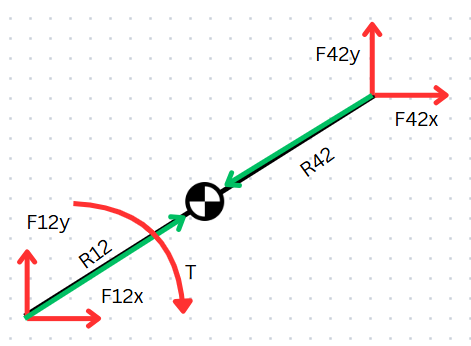
\includegraphics[width=0.85\linewidth,height=0.29\textheight,keepaspectratio]{figures/rId19.png}\par

\caption{Free-body diagram of member 2.}\end{figure}

\begin{center}\begin{adjustbox}{max width=\linewidth}$\displaystyle Link 2:\left\{ \begin{gathered}{F}_{12}^{x}+{F}_{42}^{x}={m}_{2}{A}_{{G}_{2}}^{x}\\{F}_{12}^{y}+{F}_{42}^{y}-{w}_{2}={m}_{2}{A}_{{G}_{2}}^{y}\\-{F}_{42}^{y}{R}_{42}^{x}+{F}_{42}^{x}{R}_{42}^{y}+{F}_{12}^{x}{R}_{12}^{y}-{F}_{12}^{y}{R}_{12}^{x}+T={I}_{2}{\alpha }_{2}\end{gathered}\right.$\end{adjustbox}\end{center}

\textbf{Member 3}

\begin{figure}[H]\centering

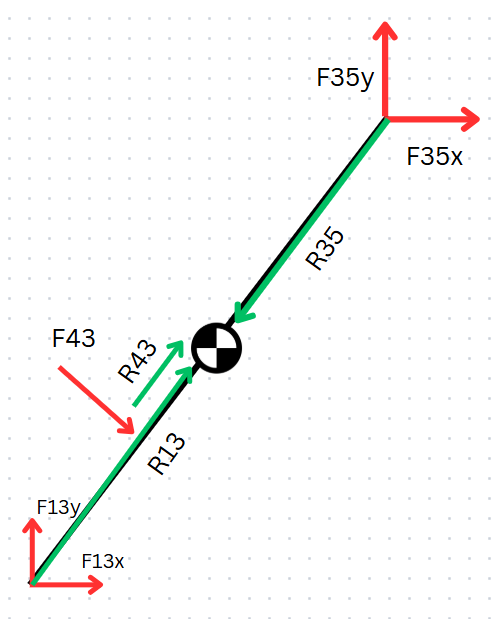
\includegraphics[width=0.85\linewidth,height=0.29\textheight,keepaspectratio]{figures/rId20.png}\par

\caption{Free-body diagram of member 3.}\end{figure}

\begin{center}\begin{adjustbox}{max width=\linewidth}$\displaystyle Link 3:\left\{ \begin{gathered}{F}_{13}^{x}+{F}_{35}^{x}+{F}_{43}^{x}={m}_{2}{A}_{{G}_{3}}^{x}\\{F}_{13}^{y}+{F}_{35}^{y}+{F}_{43}^{y}-{w}_{3}={m}_{2}{A}_{{G}_{3}}^{y}\\+{F}_{35}^{y}{R}_{35}^{x}-{F}_{35}^{x}{R}_{35}^{y}+{F}_{13}^{x}{R}_{13}^{y}-{F}_{13}^{y}{R}_{13}^{x}+{F}_{43}^{x}{R}_{43}^{y}+{F}_{43}^{y}{R}_{43}^{x}={I}_{3}{\alpha }_{3}\\{F}_{43}^{x}cos{\bar{\theta }}_{3}-{F}_{43}^{y}sin{\bar{\theta }}_{3}=0\end{gathered}\right.$\end{adjustbox}\end{center}

\textbf{Member 4}

\begin{figure}[H]\centering

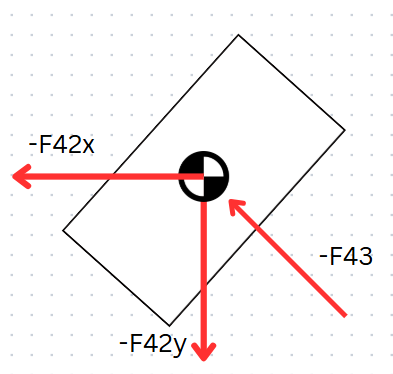
\includegraphics[width=0.85\linewidth,height=0.29\textheight,keepaspectratio]{figures/rId21.png}\par

\caption{Free-body diagram of slider 4.}\end{figure}

\begin{center}\begin{adjustbox}{max width=\linewidth}$\displaystyle Link 4:\left\{ \begin{gathered}-{F}_{42}^{x}-{F}_{43}^{x}={m}_{4}{A}_{{G}_{4}}^{x}\\-{F}_{42}^{y}+{F}_{43}^{y}-{w}_{4}={m}_{4}{A}_{{G}_{4}}^{y}\\0+0={I}_{4}{\alpha }_{4}={I}_{4}{\alpha }_{3}\end{gathered}\right.$\end{adjustbox}\end{center}

\textbf{Member 5}

\begin{figure}[H]\centering

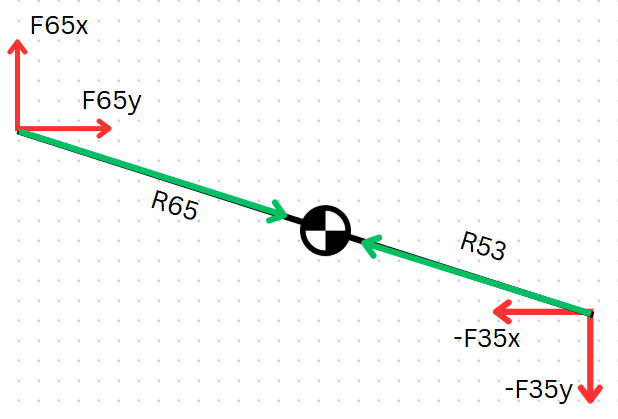
\includegraphics[width=0.85\linewidth,height=0.29\textheight,keepaspectratio]{figures/rId22.png}\par

\caption{Free-body diagram of member 5.}\end{figure}

\begin{center}\begin{adjustbox}{max width=\linewidth}$\displaystyle Link 5:\left\{ \begin{gathered}-{F}_{35}^{x}+{F}_{65}^{x}={m}_{5}{A}_{{G}_{5}}^{x}\\-{F}_{35}^{y}+{F}_{65}^{y}-{w}_{5}={m}_{5}{A}_{{G}_{5}}^{y}\\-{F}_{35}^{x}{R}_{35}^{y}-{F}_{35}^{y}{R}_{35}^{x}-{F}_{65}^{x}{R}_{65}^{y}-{F}_{65}^{y}{R}_{65}^{x}={I}_{5}{\alpha }_{5}\end{gathered}\right.$\end{adjustbox}\end{center}

\textbf{Member 6}

\begin{figure}[H]\centering

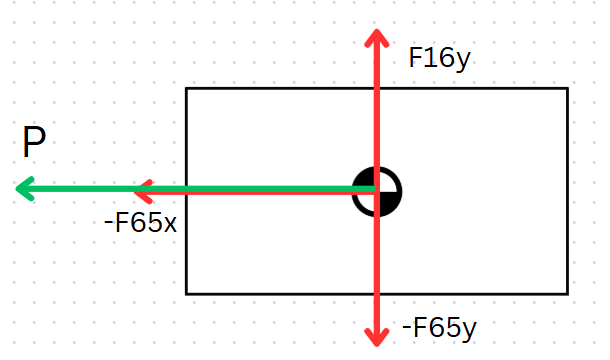
\includegraphics[width=0.85\linewidth,height=0.29\textheight,keepaspectratio]{figures/rId23.png}\par

\caption{Free-body diagram of slider 6.}\end{figure}

\begin{center}\begin{adjustbox}{max width=\linewidth}$\displaystyle Link 6:\left\{ \begin{gathered}-P-{F}_{65}^{x}={m}_{6}{A}_{{G}_{6}}^{x}\\{F}_{16}^{y}-{F}_{65}^{y}-{w}_{6}=0\\0+0=0\end{gathered}\right.$\end{adjustbox}\end{center}

Member masses and moments of inertia are obtained from Adams. The source assigns a density of 1 kg/m$^3$ and reads Calculated Mass and IZZ from the information dialog.

\begin{figure}[H]\centering

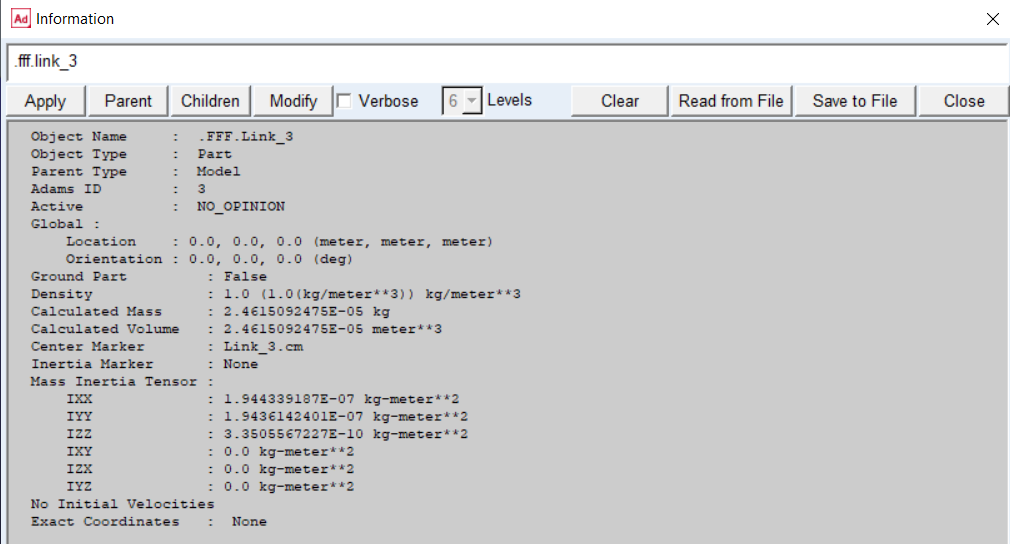
\includegraphics[width=0.85\linewidth,height=0.29\textheight,keepaspectratio]{figures/rId24.png}\par

\caption{Member properties displayed in Adams.}\end{figure}

The dynamic system has fourteen equations and fourteen unknowns. A coefficient matrix is assembled to solve the force and torque components.

\begin{center}\begin{adjustbox}{max width=\linewidth}$\displaystyle \left[ \begin{matrix}1 & 1 & 0 & 0 & 0 & 0 & 0 & 0 & 0 & 0 & 0 & 0 & 0 & 0\\0 & 0 & 1 & 1 & 0 & 0 & 0 & 0 & 0 & 0 & 0 & 0 & 0 & 0\\{R}_{12}^{y} & {R}_{42}^{y} & -{R}_{12}^{x} & -{R}_{42}^{x} & 1 & 0 & 0 & 0 & 0 & 0 & 0 & 0 & 0 & 0\\0 & 0 & 0 & 0 & 0 & 1 & 1 & 1 & 0 & 0 & 0 & 0 & 0 & 0\\0 & 0 & 0 & 0 & 0 & 0 & 0 & 0 & 1 & 1 & -1 & 0 & 0 & 0\\0 & 0 & 0 & 0 & 0 & {R}_{13}^{y} & -{R}_{35}^{y} & {R}_{43}^{y} & -{R}_{13}^{x} & {R}_{35}^{x} & {R}_{43}^{x} & 0 & 0 & 0\\0 & 0 & 0 & 0 & 0 & 0 & 0 & cos{\bar{\theta }}_{3} & 0 & 0 & -sin{\bar{\theta }}_{3} & 0 & 0 & 0\\0 & -1 & 0 & 0 & 0 & 0 & 0 & -1 & 0 & 0 & 0 & 0 & 0 & 0\\0 & 0 & 0 & -1 & 0 & 0 & 0 & 0 & 0 & 0 & 1 & 0 & 0 & 0\\0 & 0 & 0 & 0 & 0 & 0 & -1 & 0 & 0 & 0 & 0 & 1 & 0 & 0\\0 & 0 & 0 & 0 & 0 & 0 & 0 & 0 & 0 & -1 & 0 & 0 & 1 & 0\\0 & 0 & 0 & 0 & 0 & 0 & -{R}_{53}^{y} & 0 & 0 & -{R}_{53}^{x} & 0 & -{R}_{65}^{y} & -{R}_{65}^{x} & 0\\0 & 0 & 0 & 0 & 0 & 0 & 0 & 0 & 0 & 0 & 0 & -1 & 0 & 0\\0 & 0 & 0 & 0 & 0 & 0 & 0 & 0 & 0 & 0 & 0 & 0 & -1 & 1\end{matrix}\right]\left[ \begin{gathered}{F}_{12}^{x}\\{F}_{42}^{x}\\{F}_{12}^{y}\\{F}_{42}^{y}\\T\\{F}_{13}^{x}\\{F}_{35}^{x}\\{F}_{43}^{x}\\{F}_{13}^{y}\\{F}_{35}^{y}\\{F}_{43}^{y}\\{F}_{65}^{x}\\{F}_{65}^{y}\\{F}_{16}^{y}\end{gathered}\right]=\left[ \begin{gathered}{m}_{2}{A}_{{G}_{2}}^{x}\\{m}_{2}{A}_{{G}_{2}}^{y}+{w}_{2}\\{I}_{2}{\alpha }_{2}\\{m}_{3}{A}_{{G}_{3}}^{x}\\{m}_{3}{A}_{{G}_{3}}^{y}+{w}_{3}\\{I}_{3}{\alpha }_{3}\\0\\{m}_{4}{A}_{{G}_{4}}^{x}\\{m}_{4}{A}_{{G}_{4}}^{y}+{w}_{4}\\{m}_{5}{A}_{{G}_{5}}^{x}\\{m}_{5}{A}_{{G}_{5}}^{y}+{w}_{5}\\{I}_{5}{\alpha }_{5}\\{m}_{6}{A}_{{G}_{6}}^{x}+P\\{w}_{6}\end{gathered}\right]$\end{adjustbox}\end{center}

The source proposes solving the matrix equation by multiplying the inverse coefficient matrix by the known vector. Because the member-3 angle changes during motion, the system is assembled within a loop to update the angular constraint. Numerical backslash or linear-system solvers are generally preferable to explicitly forming an inverse; the supplied code includes linear solves.

\section{Cam Design}

Member 2 is removed and replaced with a cam arrangement. The supplied target-angle information, described in the source as spreadsheet data, is used to calculate the cam radius.

\subsection{Cam construction}

The instantaneous cam radius is determined from the illustrated geometric relationship between the cam and member 3.

\begin{figure}[H]\centering

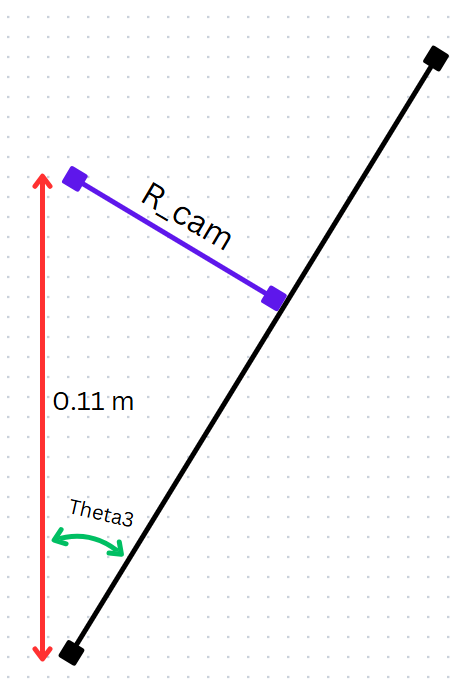
\includegraphics[width=0.85\linewidth,height=0.29\textheight,keepaspectratio]{figures/rId26.png}\par

\caption{Instantaneous cam and follower geometry.}\end{figure}

As the member-3 angle changes at each step, the corresponding cam radius changes. The given angular displacement is used in the following relation.

\begin{center}\begin{adjustbox}{max width=\linewidth}$\displaystyle {R}_{cam}=0.11\times sin{(\theta }_{3}+\psi )$\end{adjustbox}\end{center}

The radius equation is implemented in Excel to obtain the radius values.

\begin{figure}[H]\centering

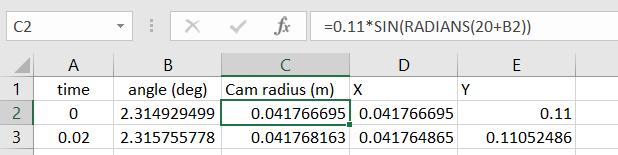
\includegraphics[width=0.85\linewidth,height=0.29\textheight,keepaspectratio]{figures/rId27.png}\par

\caption{Spreadsheet calculation of the cam radius.}\end{figure}

The coordinates of the points on the cam profile are then calculated.

\begin{figure}[H]\centering

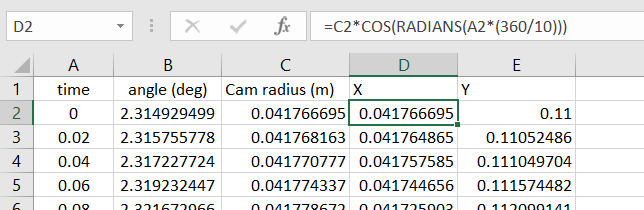
\includegraphics[width=0.85\linewidth,height=0.29\textheight,keepaspectratio]{figures/rId28.png}\par

\caption{Spreadsheet calculation of cam coordinates.}\end{figure}

The X and Y coordinates are saved as CSV data and imported into Adams. The spreadsheet and CSV are not separately included in the supplied archive; the screenshots are retained.

\begin{figure}[H]\centering

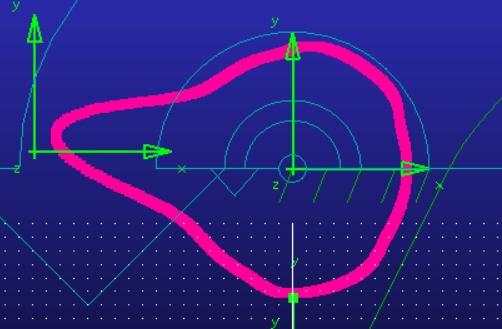
\includegraphics[width=0.85\linewidth,height=0.29\textheight,keepaspectratio]{figures/rId29.png}\par

\caption{Cam profile imported into Adams.}\end{figure}

The cam and member 3 are defined as curves and constrained using a 2D curve--curve connection. MATLAB Curve Fitter is used to approximate the target curve with an R-squared value close to one. The fitted equation is then entered into Excel to generate coordinates for the Adams geometry. The source describes the simulated follower motion as resembling the project target. A numerical error metric is not supplied.

\begin{figure}[H]\centering

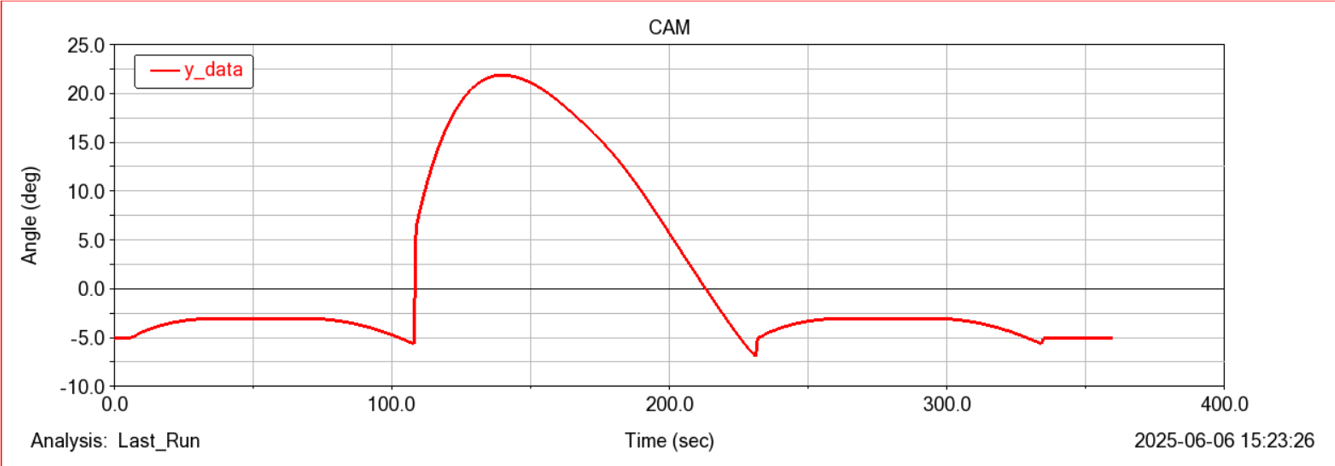
\includegraphics[width=0.85\linewidth,height=0.29\textheight,keepaspectratio]{figures/rId30.png}\par

\caption{Follower angle obtained using the cam in Adams.}\end{figure}

\section{Simulation and Comparison}

This section describes the Adams, SolidWorks, and MATLAB modeling and comparison procedure.

\subsection{Adams model}

The initial mechanism geometry is tested in Adams by trying different point locations until the arrangement shown below is obtained.

\begin{figure}[H]\centering

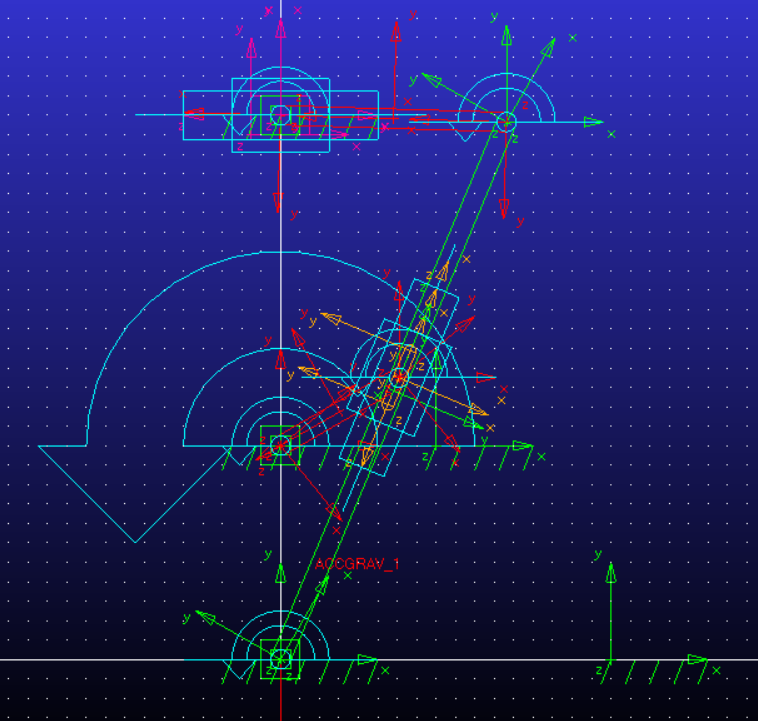
\includegraphics[width=0.85\linewidth,height=0.29\textheight,keepaspectratio]{figures/rId31.png}\par

\caption{Quick-return mechanism in Adams.}\end{figure}

The source describes prescribing crank rotation with a one-degree time-based increment and running two revolutions with 500 simulation steps. Members 2 and 4 are pinned together, while members 3 and 4 have relative sliding motion. Member 5 is pinned to member 6, and member 6 slides relative to ground. Measure definitions are used to track link angles and vector lengths over time. The exact motion-function units should be checked in the native model.

\subsection{Comparison plots}

The following plots compare the appended MATLAB analysis with Adams over two crank revolutions.

\begin{figure}[H]\centering

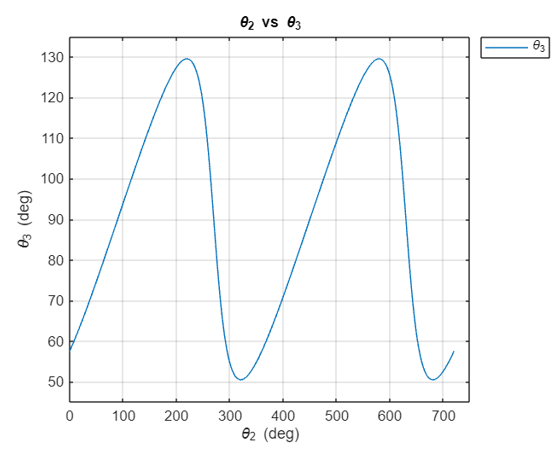
\includegraphics[width=0.85\linewidth,height=0.29\textheight,keepaspectratio]{figures/rId32.png}\par

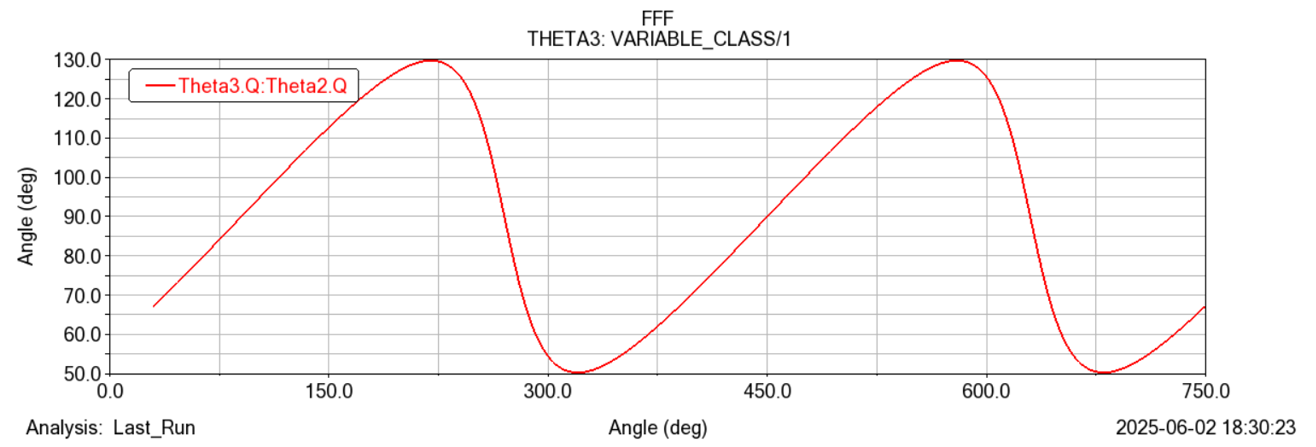
\includegraphics[width=0.85\linewidth,height=0.29\textheight,keepaspectratio]{figures/rId33.png}\par

\caption{Member 3 angular-position comparison.}\end{figure}

The source describes the member-3 angle plots as similar. Their different initial phase is attributed to MATLAB starting the crank at zero degrees and Adams starting at 30 degrees.

The member-5 angle plots are also described as similar, with the initial-angle difference discussed above.

\begin{figure}[H]\centering

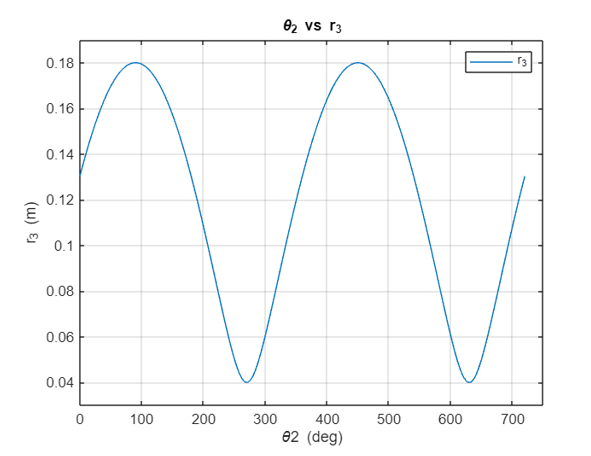
\includegraphics[width=0.85\linewidth,height=0.29\textheight,keepaspectratio]{figures/rId36.png}\par

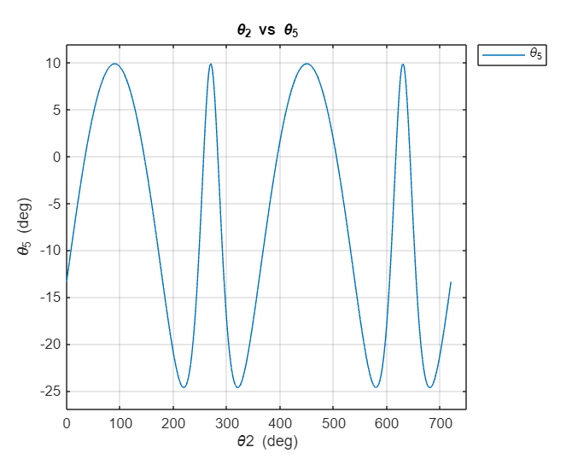
\includegraphics[width=0.85\linewidth,height=0.29\textheight,keepaspectratio]{figures/rId37.png}\par

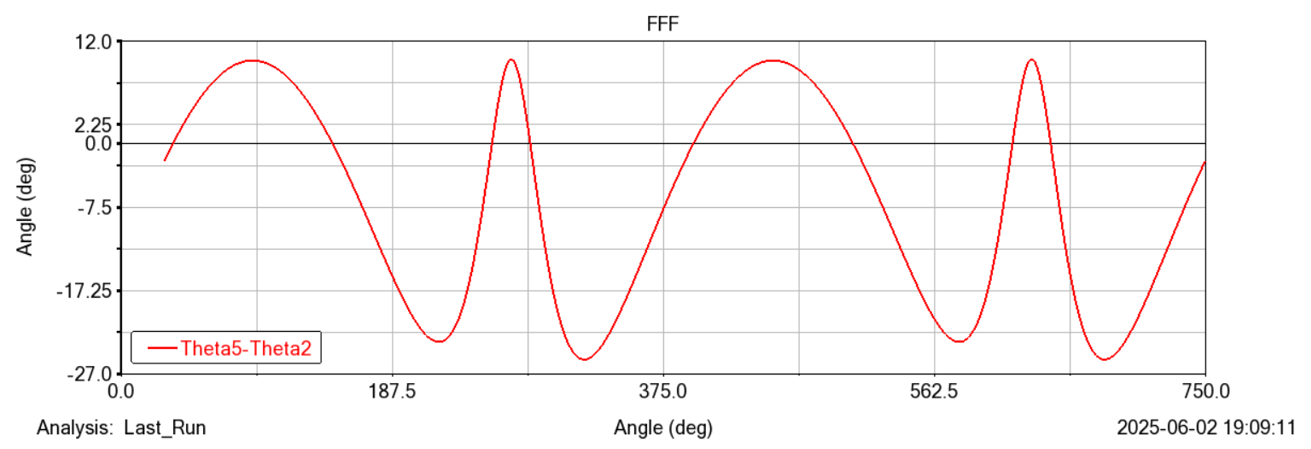
\includegraphics[width=0.85\linewidth,height=0.29\textheight,keepaspectratio]{figures/rId38.png}\par

\caption{Original figures accompanying the member 5 angle comparison.}\end{figure}

The variable vector-length plot represents the distance from slider 4 to the O3 support.

\begin{figure}[H]\centering

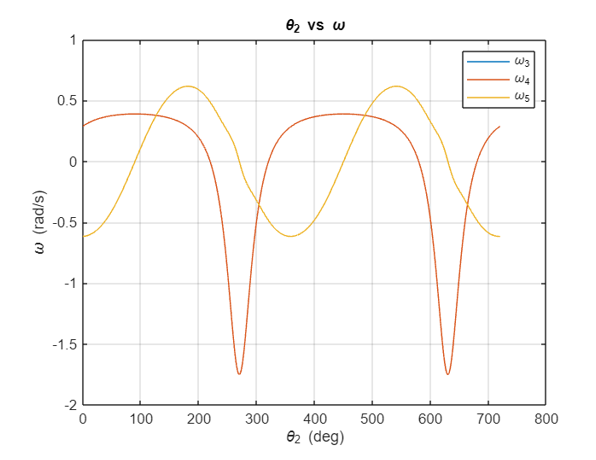
\includegraphics[width=0.85\linewidth,height=0.29\textheight,keepaspectratio]{figures/rId41.png}\par

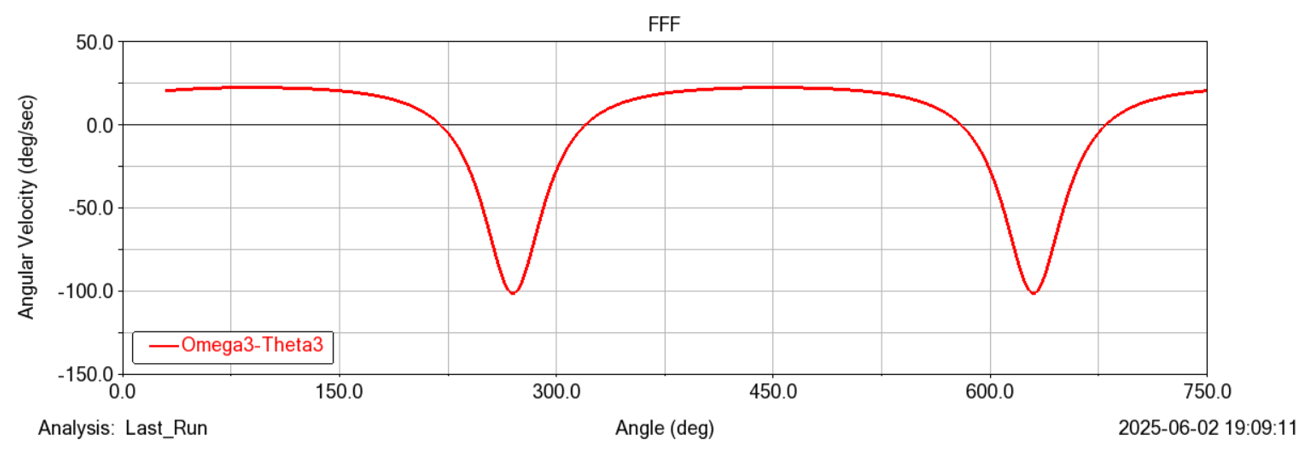
\includegraphics[width=0.85\linewidth,height=0.29\textheight,keepaspectratio]{figures/rId42.png}\par

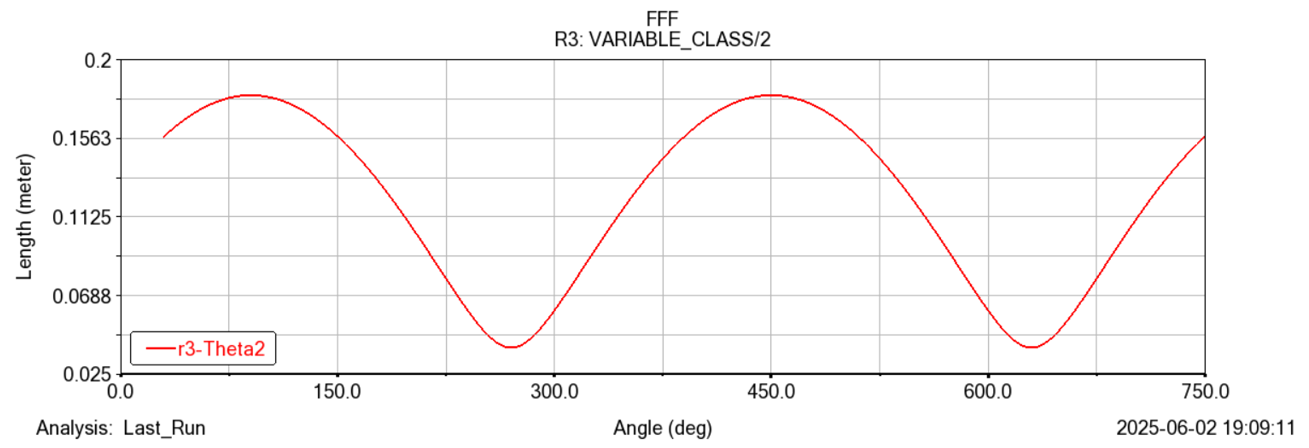
\includegraphics[width=0.85\linewidth,height=0.29\textheight,keepaspectratio]{figures/rId45.png}\par

\caption{Original figures accompanying the variable-length comparison.}\end{figure}

The member-3 angular velocities are described as similar, but member 5's angular velocity does not agree. The source suspects an error in assembling the MATLAB equations. It notes that the following acceleration comparison appears similar, but that observation alone does not prove the velocity discrepancy has been resolved. The member-3 and member-4 curves overlap in the MATLAB velocity plot because those members share angular motion; the same observation is made for angular acceleration.

\begin{figure}[H]\centering

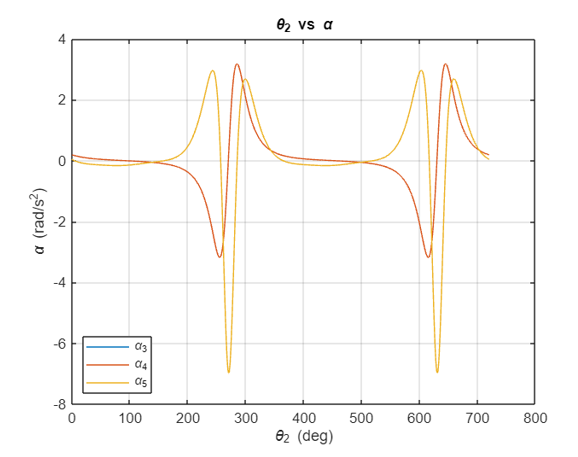
\includegraphics[width=0.85\linewidth,height=0.29\textheight,keepaspectratio]{figures/rId46.png}\par

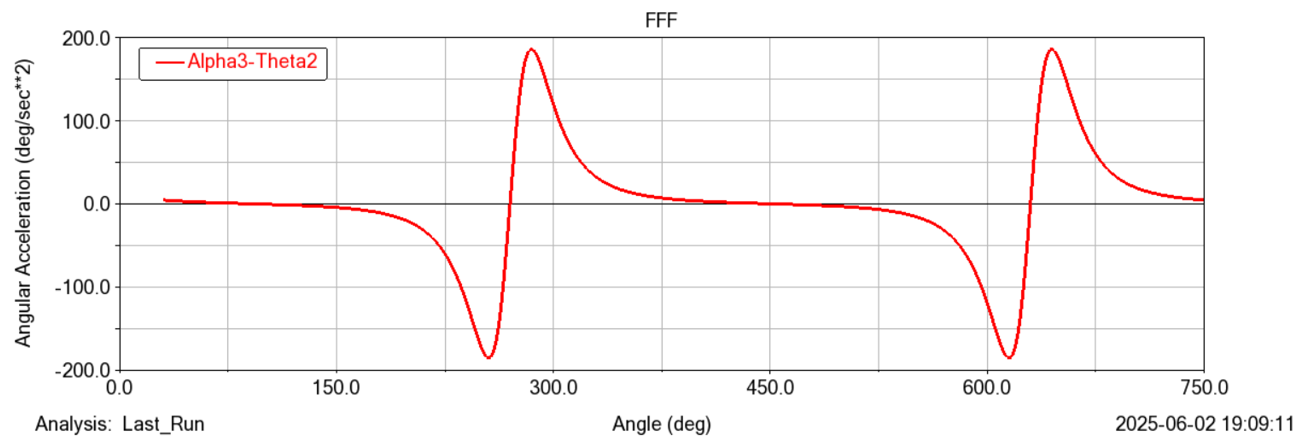
\includegraphics[width=0.85\linewidth,height=0.29\textheight,keepaspectratio]{figures/rId47.png}\par

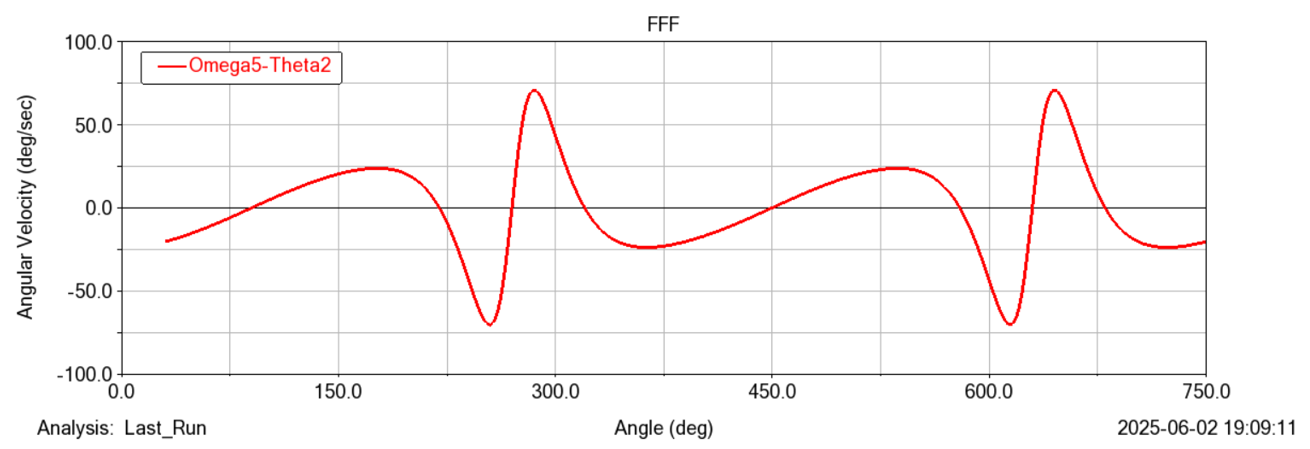
\includegraphics[width=0.85\linewidth,height=0.29\textheight,keepaspectratio]{figures/rId50.png}\par

\caption{Angular-velocity comparison figures.}\end{figure}

The source states that the angular-acceleration plots appear similar despite the discrepancy in member-5 angular velocity. Original figures are retained as supplied; one figure in this location is labeled as a force plot rather than an angular-acceleration plot.

\begin{figure}[H]\centering

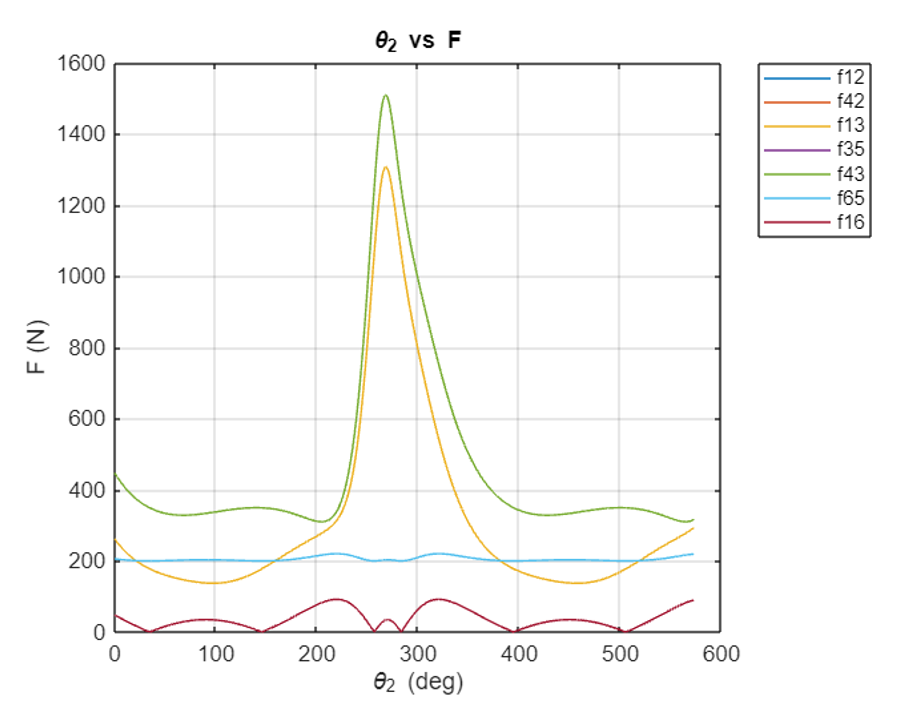
\includegraphics[width=0.85\linewidth,height=0.29\textheight,keepaspectratio]{figures/rId51.png}\par

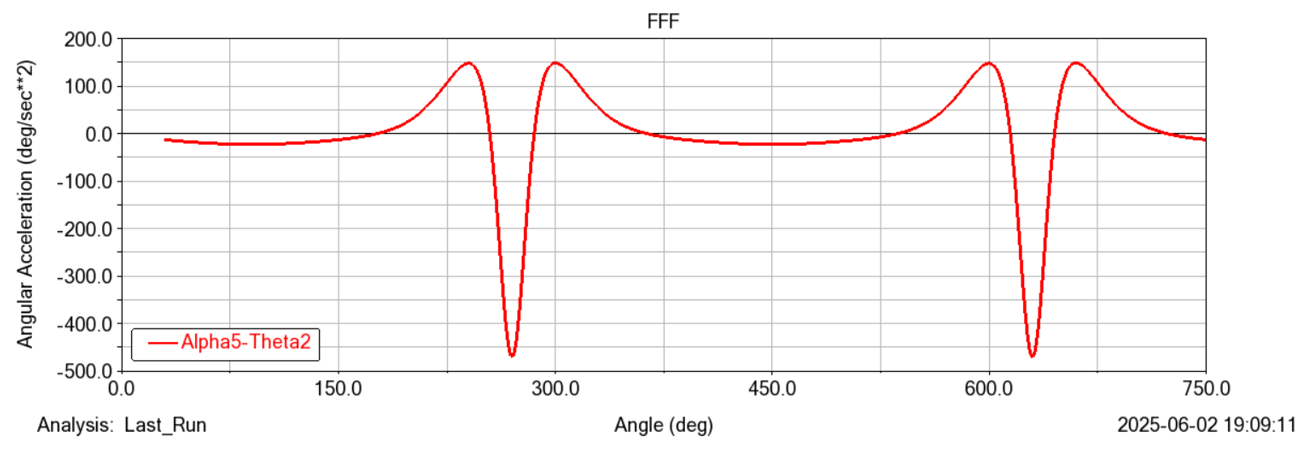
\includegraphics[width=0.85\linewidth,height=0.29\textheight,keepaspectratio]{figures/rId52.png}\par

\caption{Original figures accompanying the acceleration comparison; one is labeled as a force plot.}\end{figure}

The following discussion concerns the force histories over the nominal ten-second interval. The source places the corresponding plots in its appendix; they are reproduced there in this edition.

The source identifies the largest forces in the approximate crank-angle range 250--350 degrees, where output slider 6 is pulled rapidly backward and decelerates. It attributes the force increase to this change in motion and describes slider 6 as the heaviest member. The saved mass assumptions should be checked before adopting that description.

The source attributes the input-torque peak to the same motion phase as the force increase.

\begin{figure}[H]\centering

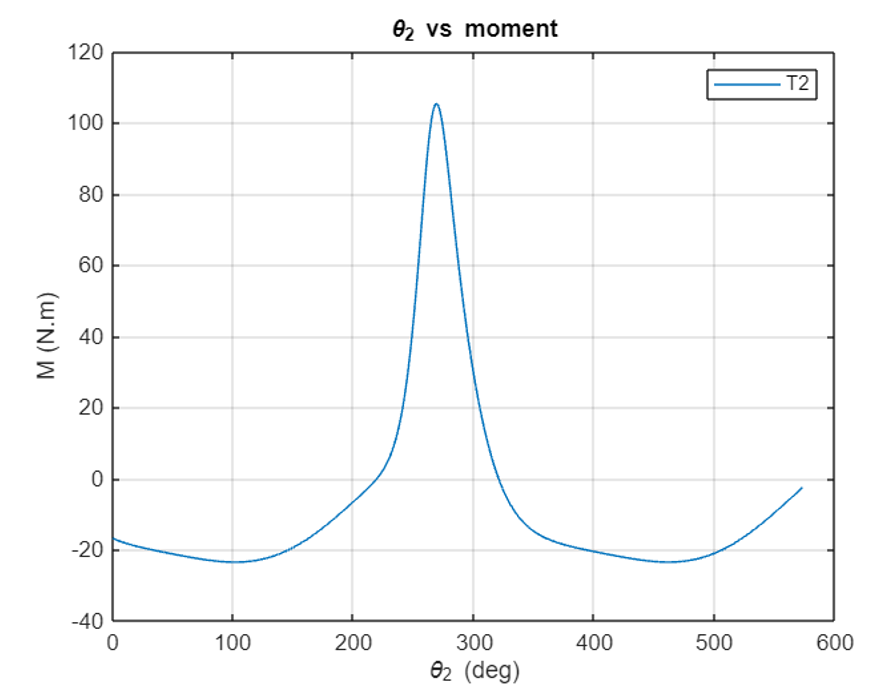
\includegraphics[width=0.85\linewidth,height=0.29\textheight,keepaspectratio]{figures/rId53.png}\par

\caption{Input-torque history.}\end{figure}

A plot is also obtained for the designed cam radius.

\begin{figure}[H]\centering

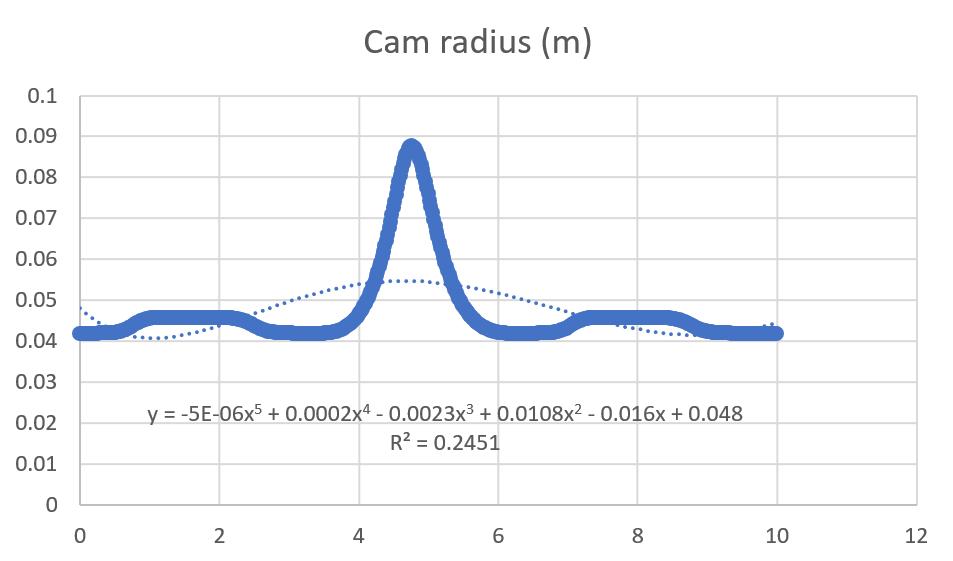
\includegraphics[width=0.85\linewidth,height=0.29\textheight,keepaspectratio]{figures/rId54.png}\par

\caption{Cam-radius plot.}\end{figure}

\subsection{SolidWorks design}

A SolidWorks model is created to determine initial dimensions and angles and to visualize the mechanism more clearly.

A ground support is included to make the assembly more representative. The holes in the links represent pin joints and have a diameter of 8 mm.

\begin{figure}[H]\centering

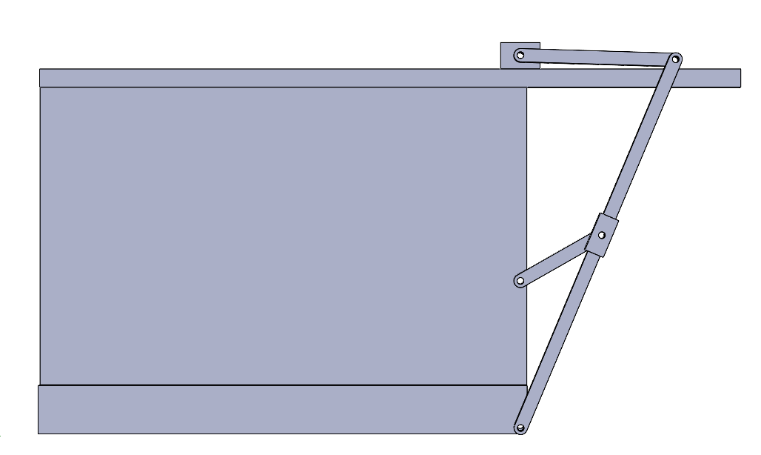
\includegraphics[width=0.85\linewidth,height=0.29\textheight,keepaspectratio]{figures/rId55.png}\par

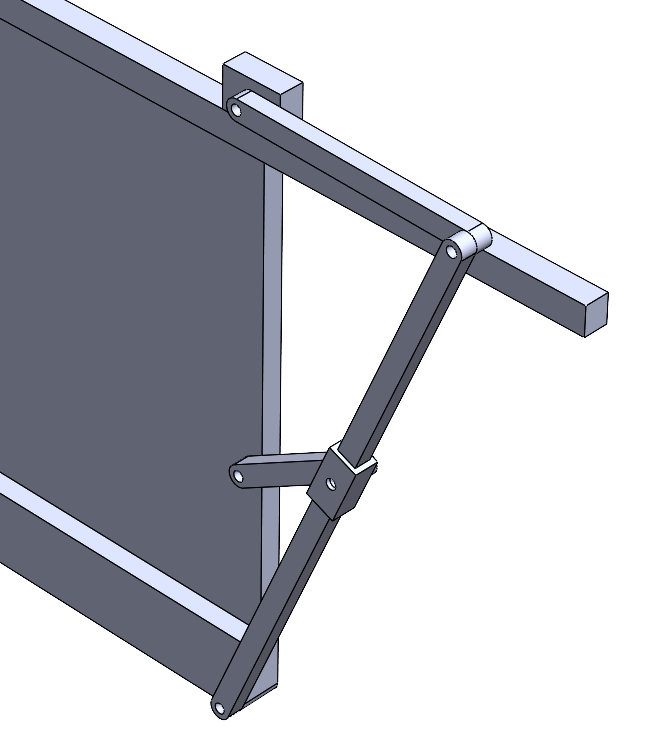
\includegraphics[width=0.85\linewidth,height=0.29\textheight,keepaspectratio]{figures/rId56.png}\par

\caption{SolidWorks mechanism model.}\end{figure}

\begin{figure}[H]\centering

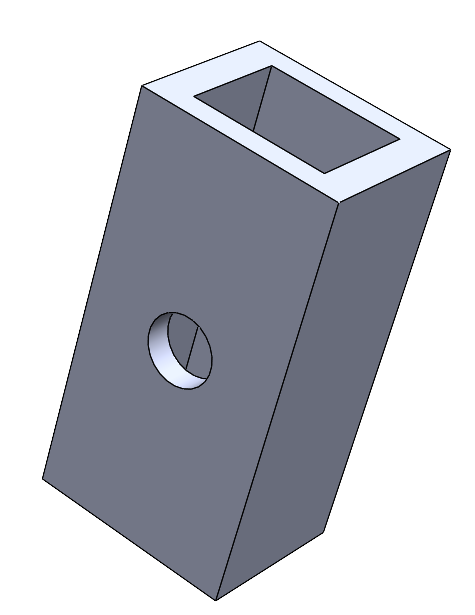
\includegraphics[width=0.85\linewidth,height=0.29\textheight,keepaspectratio]{figures/rId59.png}\par

\caption{Slider 4 geometry.}\end{figure}

The slider opening is 10 by 8 mm, matching the cross section of member 3 along which it slides. An animation of this assembly is included in the archive. Manufacturing clearances are not established by the nominal dimensions alone.

\section{Conclusion}

The project examines the kinematic and dynamic behavior of a quick-return mechanism through analytical modeling and software simulation. A MATLAB program calculates and plots angular velocities and accelerations. The source concludes that the selected geometry supports complete continuous motion.

Joint forces and input torque are calculated for the stated loading conditions. The source interprets the results as predictable operation of the mechanism and describes the cam-based alternative as reproducing the desired motion. These are the author's interpretations of the software study, subject to the unresolved comparison and model issues noted in this edition.

Quick-return mechanisms offer a simple way to obtain controlled reciprocating motion. Appropriate design may reduce cycle time and improve machine operation, although this project does not provide a quantified energy-efficiency optimization.

The study illustrates the use of analytical methods alongside simulation in mechanism design. Future work could examine friction and vibration to obtain a more realistic model.

\section{References}

Machine Dynamics teaching-assistant project instructions, School of Mechanical Engineering. Not supplied as a separate file.

Robert L. Norton, Design of Machinery, third edition, McGraw-Hill, 2004. Citation retained from the source report.

\FloatBarrier\appendix\section{MATLAB Source Listing}
The listing below is extracted from the original report. Section headings are comments; the numerical logic is retained. The native Live Script is supplied separately and may contain a different saved revision.
\lstinputlisting{../matlab/report_listing.m}
\section{Original Appendix Output Figures}


\begin{figure}[H]\centering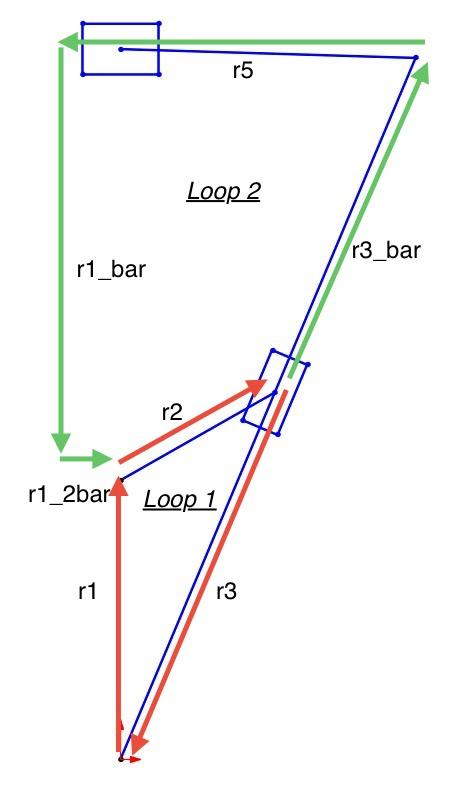
\includegraphics[width=0.90\linewidth,height=0.32\textheight,keepaspectratio]{figures/rId60.png}\caption{Original MATLAB appendix output 60.}\end{figure}

\begin{figure}[H]\centering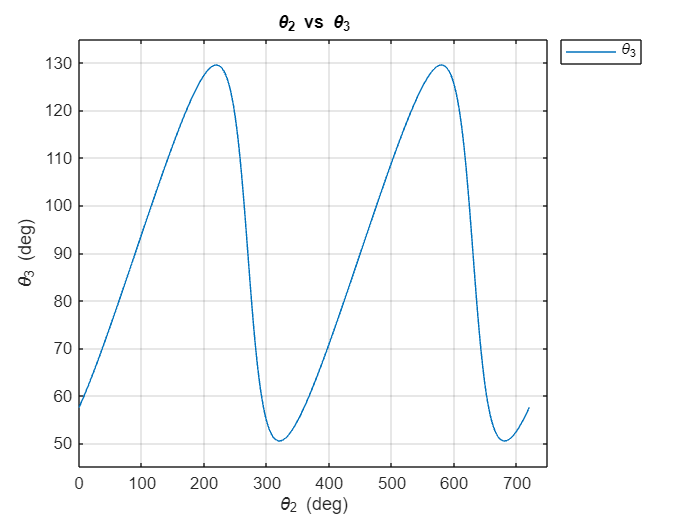
\includegraphics[width=0.90\linewidth,height=0.32\textheight,keepaspectratio]{figures/rId61.png}\caption{Original MATLAB appendix output 61.}\end{figure}

\begin{figure}[H]\centering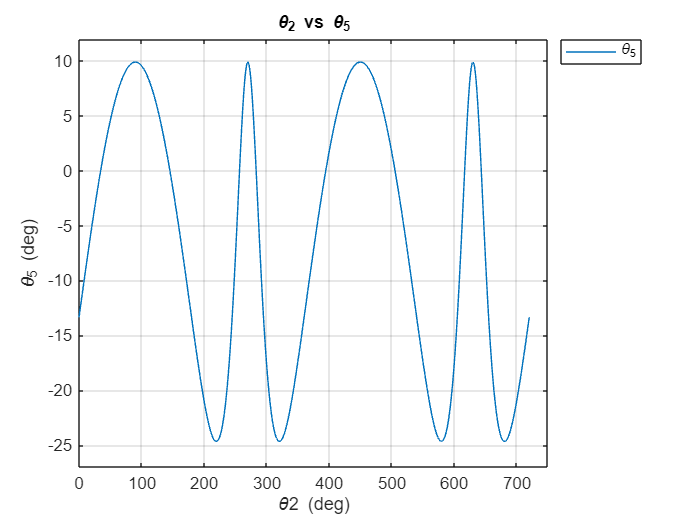
\includegraphics[width=0.90\linewidth,height=0.32\textheight,keepaspectratio]{figures/rId62.png}\caption{Original MATLAB appendix output 62.}\end{figure}

\begin{figure}[H]\centering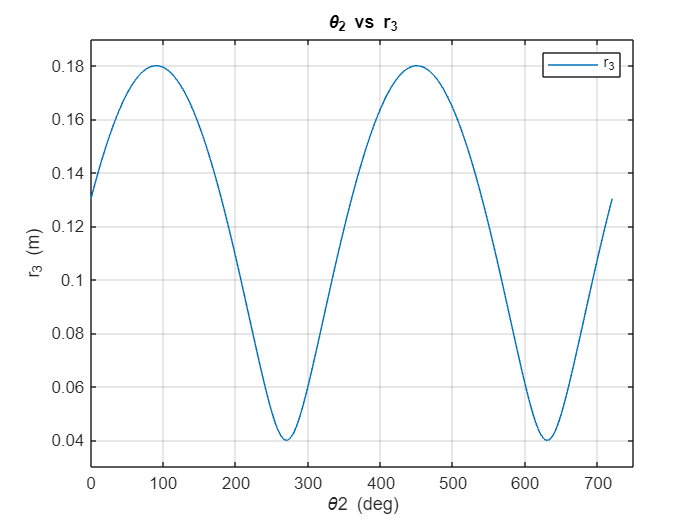
\includegraphics[width=0.90\linewidth,height=0.32\textheight,keepaspectratio]{figures/rId63.png}\caption{Original MATLAB appendix output 63.}\end{figure}

\begin{figure}[H]\centering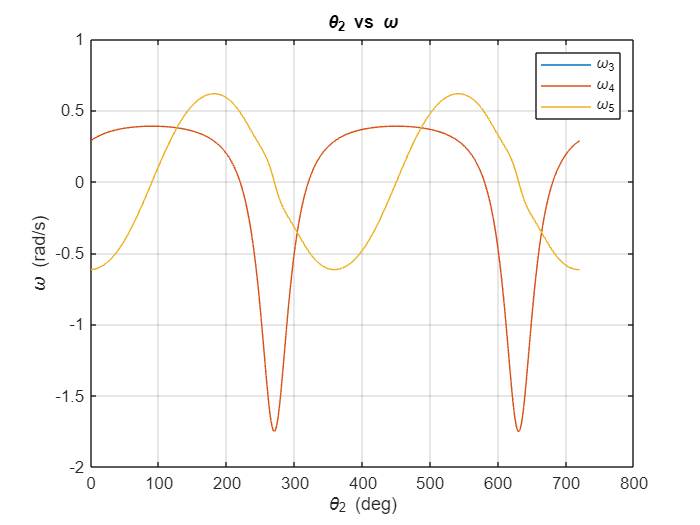
\includegraphics[width=0.90\linewidth,height=0.32\textheight,keepaspectratio]{figures/rId64.png}\caption{Original MATLAB appendix output 64.}\end{figure}

\begin{figure}[H]\centering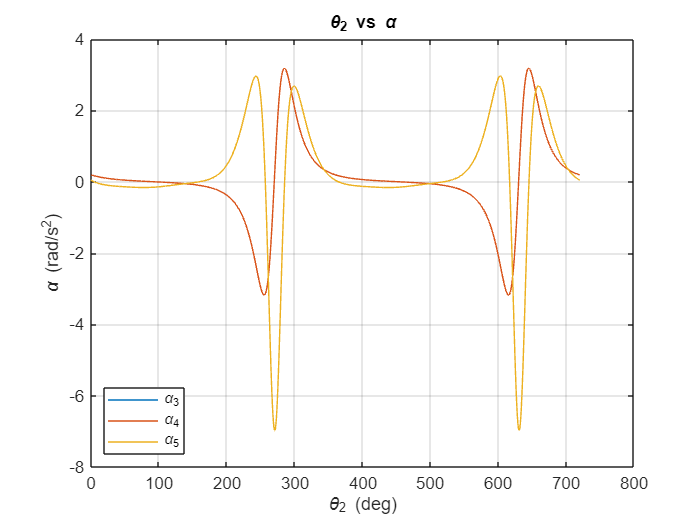
\includegraphics[width=0.90\linewidth,height=0.32\textheight,keepaspectratio]{figures/rId65.png}\caption{Original MATLAB appendix output 65.}\end{figure}

\begin{figure}[H]\centering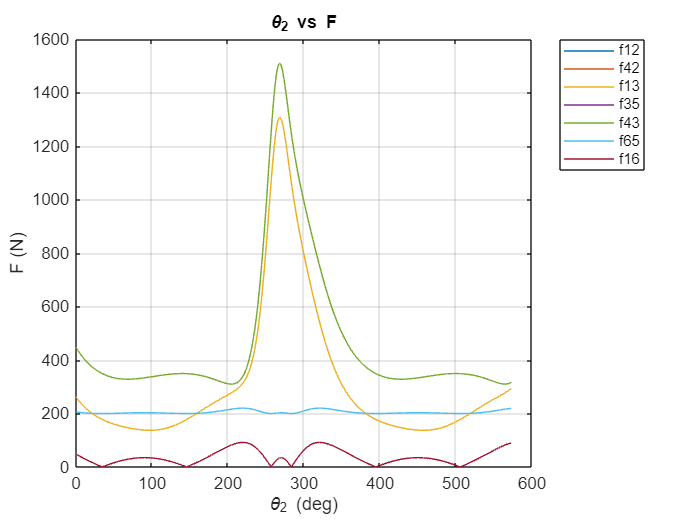
\includegraphics[width=0.90\linewidth,height=0.32\textheight,keepaspectratio]{figures/rId66.png}\caption{Original MATLAB appendix output 66.}\end{figure}

\begin{figure}[H]\centering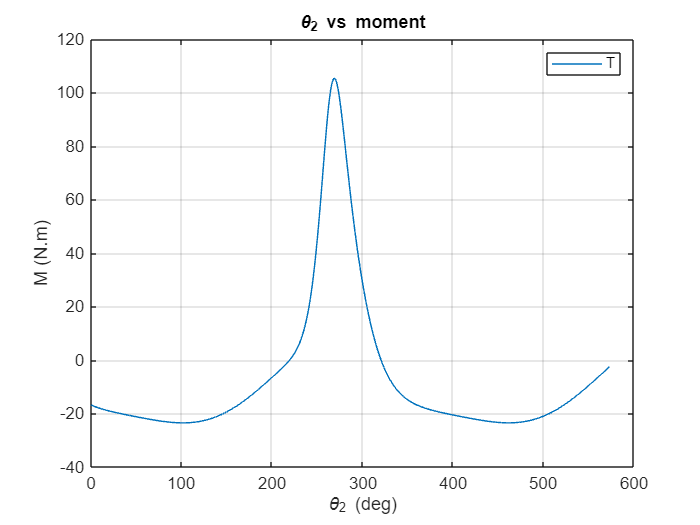
\includegraphics[width=0.90\linewidth,height=0.32\textheight,keepaspectratio]{figures/rId67.png}\caption{Original MATLAB appendix output 67.}\end{figure}

\begin{figure}[H]\centering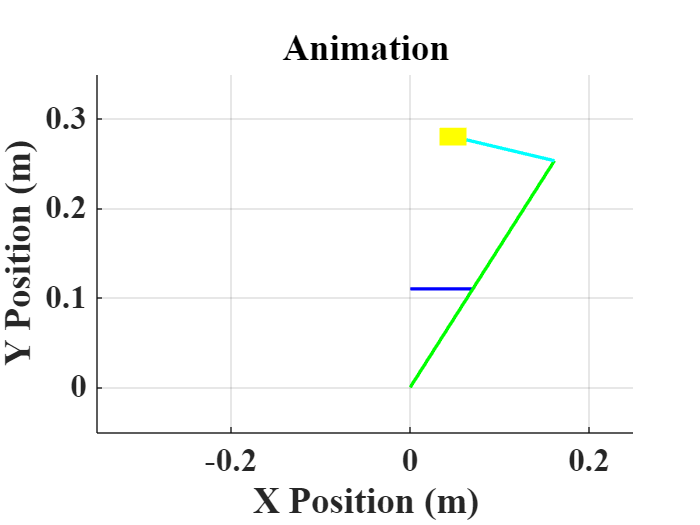
\includegraphics[width=0.90\linewidth,height=0.32\textheight,keepaspectratio]{figures/rId68.png}\caption{Original MATLAB appendix output 68.}\end{figure}

\FloatBarrier\section{Editorial Review and Reproducibility}
The original study provides software comparisons, not experimental validation or a quantified optimization objective. The observed member-5 angular-velocity mismatch remains unresolved. Similar-looking acceleration curves do not establish that the velocity equation is correct.

The MATLAB source merits review before reuse. In the second-loop velocity right-hand side, several displacement and derivative terms appear inside the sine/cosine arguments instead of being added as separate terms. In the first-loop acceleration expression, a term uses r3p where the expected radial centripetal term warrants checking against r3. The dynamic member-5 force equations use aG4x and aG4y rather than the separately calculated member-5 accelerations. These are inspection findings, not fixes that have been validated by a rerun.

The source assigns a density of 1 kg/m$^3$ and uses correspondingly small masses and inertias. These are modeling assumptions, not established material properties for the CAD parts. The statement that slider 6 is the heaviest member should be checked against the supplied mass list. Gravity, the 200 N load, coordinate signs, and mass units must be consistent between programs. Some report equations contain inconsistent subscripts and signs. The fourteen-equation matrix is retained as a source transcription; do not treat it as a verified implementation independent of the code.

The MATLAB study uses 2000 points over $0\le\theta_2\le4\pi$, with input speed 1 rad/s and zero angular acceleration. The nominal two-cycle kinematic interval is therefore about 12.57 seconds. The dynamic subsection uses a shorter interval and a hardcoded plotting index; distinguish angle axes from time histories when comparing figures. The source's Adams description of a degree-based time increment is not a confirmed identical speed setting.

The original MATLAB Live Script and workspace, Adams binary models, SAM project, SolidWorks assembly and referenced parts, and available smaller videos are included. The Excel cam worksheet, coordinate CSV, and a separate curve-fit export are not supplied. Their screenshots are retained, but missing numerical source data have not been reconstructed. MATLAB requires Symbolic Math Toolbox for the symbolic expressions and matrix generation. A compatible release is needed for local functions placed amid script sections; the native Live Script is the preferred starting point.

The extracted text version preserves code blocks and turns Live Script prose headings into comments. It does not reproduce stored Live Editor output or embedded illustrations and is not claimed to be a tested standalone replacement. The report listing is a second historical source and may differ from the saved Live Script. Original files have not been altered.

Adams native models are compressed together in \texttt{adams/native\_models.zip} to keep each browser-uploaded file within GitHub's 25 MiB limit. Extract that archive before opening the models. The approximately 62.4 MiB MATLAB video is omitted from this repository package and remains in the original RAR archive; it is not required to build the report. All other supplied videos are included. No native CAD rebuild, multibody rerun, or hardware experiment was performed during preparation.
\end{document}